\section {Photonik}
\subsection {Grundlagen}
\subsubsection {Der Begriff Photonik}
Unter Photonik (englisch: photonics) wird die Gesamtheit der optischen Techniken verstanden, mit der Licht erzeugt, verstärkt, geformt, übertragen, gemessen und als elektromagnetische Strahlung nutzbar gemacht wird. Basis für diese neuen Werkzeuge aus Licht sind die klassische Optik, die Optoelektronik und Lasertechnik. Durch die fast grenzenlosen Einsatzmöglichkeiten ist Photonik zur Querschnitts-und Schlüsseltechnologie geworden. Die auch als optische Technologien bezeichneten Produkte werden in Autos, Computern, CD-Playern, Handys, Fernbedienungen, in der Kommunikationstechnik, beim Röntgen oder in der industriellen Fertigungstechnik eingesetzt. Kernprodukte wie Laser oder Glasfasern machen andere Innovationen erst möglich.

\subsection {Physikalische Grundlagen}
\subsubsection {Elektromagnetische Strahlung}
Licht ist der für das Auge sichtbare Teil der elektromagnetischen Strahlung. Im elektromagnetischen Spektrum umfasst der Bereich des Lichts Wellenlängen von etwa 380 nm bis 780 nm. Elektromagnetische Strahlung existiert aber in einem wesentlich grösseren Frequenzbereich. Nur ein kleiner Frequenzbereich ist für Menschen sichtbar.
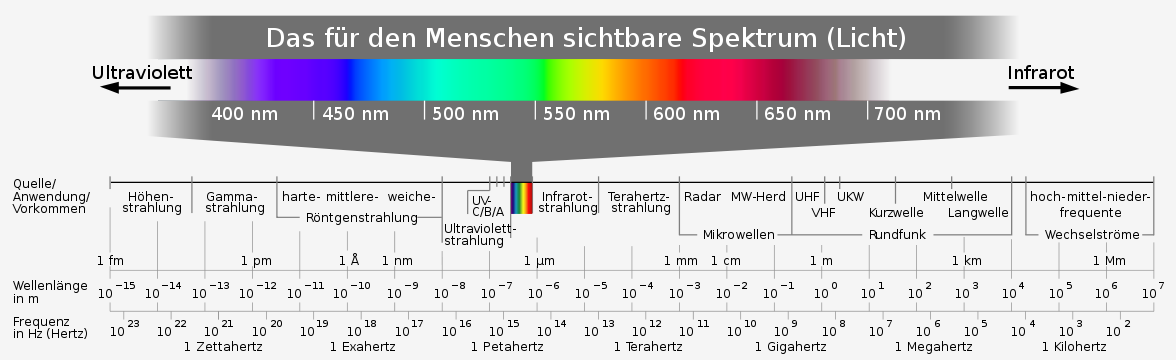
\includegraphics[width=\textwidth]{images/strahlung}

\begin{multicols}{2}
\paragraph {Lichtgeschwindigkeit im Vakuum}
$c = \frac {1}{\sqrt{\mu_0 \epsilon_0}} = 299792458 \frac{m}{s}$

\paragraph {Lichtgeschwindigkeit im Medium}
$c = \frac {1}{\sqrt{\mu_0 \mu_r \epsilon_0 \epsilon_r}}$ auf Leiterplatte $c = 20 \frac{cm}{ns}$ 
\end{multicols}

\paragraph {Photonen}
Licht besteht aus diskreten Energiequanten, den so genannten Photonen.
\begin{multicols}{3}
Energie: \\ $E = h * v$ \\
Plancksche Wirkungsquantum: \\ $h = 6.62606957 * 10^{-34} Js$ \\
Impuls: \\ $p = \frac {h}{\lambda}$ 
\end{multicols}

\subsubsection {Photoeffekt}
\begin{multicols}{4}
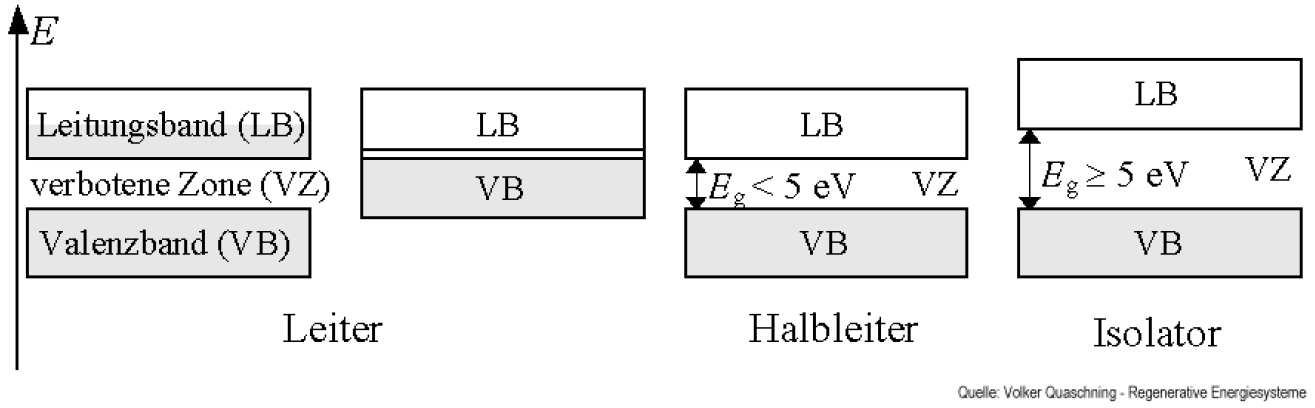
\includegraphics[width=0.5\textwidth]{images/Leitungsband} \\ \columnbreak 
\ \\ \vfill \columnbreak 
Mit der Energie des Lichtes kann ein Elektron auf eine höhere Bahn gehoben werden oder auch herausgeschlagen werden. \\ 
$E = \frac{h * c}{\lambda}$
\end{multicols}

\paragraph{äusserer Photoelektrischer Effekt}
Herauslösen von Elektronen aus einer Halbleiter- oder Metalloberfläche, benötigt eine hohe Ionisationsenergie.

\paragraph{innerer Photoelektrischer Effekt}
Silizium weist eine Bandlücke von 1.1eV auf zwischen dem Leitungs- und dem Valenz-Band. Damit ein Elektron den Sprung ins Leitungsband schafft, muss es die Energie von mindestens 1.1eV aufnehmen. Hat ein Photon diese oder eine grössere Energie, kann eine Wechselwirkung auftreten: Das Photon wird absorbiert, das Elektron springt ins Leitungsband und ein Loch bleibt zurück. Trifft ein Photon mit geringerer Energie auf den Silizium-Kristall, gibt es keine Wechselwirkung und das Photon fliegt durch den Kristall hindurch. Weist das Photon eine höhere Energie auf, so wird es absorbiert und die überschüssige Energie verpufft.

